\documentclass[10pt,conference]{IEEEtran}

% Paquetes
\usepackage[utf8]{inputenc}
\usepackage[spanish,es-tabla]{babel} % Idioma español con tablas
\usepackage{apacite} % Referencias y Citas
\usepackage{float} % Para var H, figure
\usepackage{graphicx}  % Paquete para insertar figuras
\usepackage{subfigure} % imagenes multiples
\usepackage{url}
\usepackage{amsmath}%Paquete para insertar símbolos matemáticos
%---------- pie de pagina
\usepackage{fancyhdr}
\pagestyle{fancy}
\fancyhf{}
\rfoot[]{\thepage}
%-----------------

%-------------------------------------------------------------
% APA7 CITAS
% \citeA{autor} -> Autor (año)
% \cite[p.~11]{autor}. cita corta -40 words -> (Autor, año, página)
%-------------------------------------------------------------

%Para alinear 4 y 5 autor.
\makeatletter
\newcommand{\newlineauthors}{%
  \end{@IEEEauthorhalign}\hfill\mbox{}\par
  \mbox{}\hfill\begin{@IEEEauthorhalign}}
\makeatother
%----------------------------------------------

\title{Aplicaciones de las expresiones regulares y autómatas finitos en la Industria}

\author{\IEEEauthorblockN{1\textsuperscript{ero} Fabricio Julian}
\IEEEauthorblockA{\textit{Escuela de Informática} \\
\textit{Universidad Nacional de Trujillo}\\
Trujillo, Perú \\
t452700220@unitru.edu.pe}
\and
\IEEEauthorblockN{2\textsuperscript{do} Angely Mendez}
\IEEEauthorblockA{\textit{Escuela de Informática} \\
\textit{Universidad Nacional de Trujillo}\\
Trujillo, Perú \\
t052701020@unitru.edu.pe}
\and
\IEEEauthorblockN{3\textsuperscript{ero} Ciara Mendez}
\IEEEauthorblockA{\textit{Escuela de Informática} \\
\textit{Universidad Nacional de Trujillo}\\
Trujillo, Perú \\
t022700920@unitru.edu.pe}
\and
\newlineauthors
\IEEEauthorblockN{4\textsuperscript{to} Valentina Padilla}
\IEEEauthorblockA{\textit{Escuela de Informática} \\
\textit{Universidad Nacional de Trujillo}\\
Trujillo, Perú \\
t032700320@unitru.edu.pe}
\and
\noindent
\IEEEauthorblockN{5\textsuperscript{to} Angie Recalde}
\IEEEauthorblockA{\textit{Escuela de Informática} \\
\textit{Universidad Nacional de Trujillo}\\
Trujillo, Perú \\
t512700720@unitru.edu.pe}
}

\begin{document}
\renewcommand{\BOthers}[1]{et al.\hbox{}} % Para reemplazar y cols. por et.al (=+ de 3 autores) APA7
\renewcommand{\IEEEkeywordsname}{{\bfseries Palabras claves:}} % Colocar Keywords en Spanish

\maketitle

\begin{abstract}
Este documento es una investigación sobre las diversas aplicaciones de las expresiones regulares y autómatas finitos en la industria, por lo cual, se consideró cinco ramas: Industria Natural, Industria Textil, Industria Química, Industria Ambiental e  Industria Tecnológica, en las cuales se plantean propuestas y se determinan múltiples soluciones a problemas que están presentes en el día a día a nivel mundial. En este articulo se evidencia que la teoría de expresiones regulares y autómatas finitos es útil y necesaria, además esta teoría es generadora de soluciones innovadoras y logrará computacionalmente nuevas metodologías y sistemas que contribuirán a mejorar en diversos ámbitos el mundo.
\end{abstract}

\vspace{2mm}
\begin{IEEEkeywords}
Autómatas finitos, autómatas celulares, expresiones regulares, industria, alimentaria, textil, química, ambiental y tecnológica. 
\end{IEEEkeywords}

\vspace{1mm}
\section{\textbf{Introducción}}
    La teoría de autómatas finitos consiste en modelos matemáticos de sistemas, con entradas y salidas discretas.El cual puede estar en cualquiera de un número finito de configuraciones o “estados”. El estado del sistema resume la información concerniente a entradas anteriores y que es necesaria para determinar el comportamiento para entradas posteriores. La teoría de autómatas finitos es una herramienta muy útil en lo que a ciencias de la computación compete, en mencionada ciencia también se encuentra muchos ejemplos de sistemas de estados finitos. Cabe resaltar que las aplicaciones modernas de la teoría de los autómatas y expresiones regulares van mucho más allá de las técnicas de compilación o la verificación del hardware. Utilizándose ampliamente para el modelamiento y verificación en software, sistemas distribuidos, sistemas en tiempo real o datos estructurados. En algunos casos hasta se han equipado con funciones para modelar el tiempo y las probabilidades, obteniéndose resultados fructíferos para el rendimiento.

    Por ello, en este articulo se presenta diversas aplicaciones respecto a las expresiones regulares y autómatas finitos en la Industria, el cual está organizado de la siguiente manera: en primer lugar, se explica la industria Alimentaria, con uno de sus ejemplos en la transformación de alimentos,en segundo lugar se evidencia la industria Textil, basándose en la teoría de autómatas celulares con autómatas textiles, en tercer lugar se presenta aplicaciones de la industria Química, con uno de sus casos en el reconocimiento del lenguaje por autómatas químicos no bioquímicos de los autómatas finitos a las máquinas de Turing, en cuarto lugar tenemos a la industria Ambiental donde se muestra entre sus tantos ejemplos el marco integrado para el dimensionamiento y la gestión energética de híbridos usando autómatas finitos, en quinto lugar se explica la industria Tecnológica, con una de sus aplicaciones en la optimización de hormigas con árbol de expansión, finalmente se presenta una breve conclusión.
    
\vspace{1mm}    
\section{\textbf{Aplicaciones}}

\vspace{2mm}
\subsection{\underline{\textbf{Industria Natural}}}
A través de diversos estudios a lo largo de los años el hombre ha ido entendiendo cada extensión de nuestro entorno, incluyendo el ambiente natural, donde también a través de diversos trabajos de investigación, se ha encontrado que el ambiente natural hace uso sobre la definición de autómatas de estado finito, autómatas celulares y moleculares.

\vspace{2mm}
\subsubsection{\textbf{Genética cuántica y modelos de autómatas cuánticos en la evolución de organismos y especies: }}
La investigación de \citeA{baianu2012quantum} se enfoca en la evolución de organismos y especies a través de la teoría cuántica de autómatas. La evolución de organismos y especies ocurre a través de transformaciones multimoleculares acopladas, contrario a la visión de los modelos darwinistas ``estándar'' de evolución.Durante la evolución se dan cambios fenotípicos, estos cambios se expresan cuando cambios cuánticos-moleculares se combinan con una reestructuración interna de los submódulos del genoma y las redes interactomas relacionadas ciclo y crecimiento celular. Se puede decir que la genética cuántica explica correctamente los procesos evolutivos que se inician en niveles cuántico-multimolecular y se propagan a niveles superiores de evolución de organismos y especies.

\vspace{2mm}
\subsubsection{\textbf{Cascadas moleculares autónomas para evaluación de superficies celulares: }}
Dentro de la nanotecnología de la naturaleza se tienen los autómatas moleculares, estos son mezclas de moléculas que experimentan cambios estructurales en respuesta a interacciones secuenciales con entradas. Se tienen autómatas moleculares basados en ácidos nucleicos que incluyen dispositivos moleculares de juego y autómatas de estado finito para el análisis de ácidos nucleicos. Para \citeA{rudchenko2013autonomous}, en el resultado final de un autómata molecular que completa su análisis es la presencia de una etiqueta molecular única en la superficie celular de una subpoblación específica de linfocitos dentro de células sanguíneas humanas ahora en la figura \ref{Natural1} se puede observar lo explicado anteriormente.
\begin{figure}[H]
 \begin{center}
       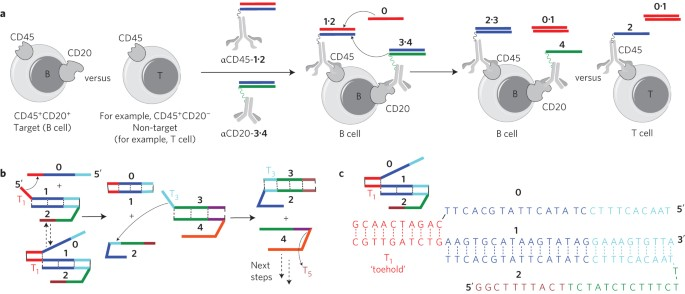
\includegraphics[width=7.5cm, height=4.5cm]{Ind. Natural/Imagen_01.jpg}
      \caption{Cascadas moleculares autónomas para evaluación de superficies celulares.}
      \label{Natural1} 
      \end{center}
\end{figure}

\vspace{2mm}
\subsubsection{\textbf{Demultiplexor molecular como autómata terminador: }}
La generación fotosensibilizada de oxígeno singlete en tumores, dentro o alrededor de las células cancerosas, es la esencia de la terapia fotodinámica del cáncer. El destino de estado excitado singlete está estrechamente relacionado con las eficiencias relativas y las velocidades de los procesos fotofísicos implicados. La eficiencia del acceso al colector triplete está directamente relacionada con el rendimiento cuántico de oxígeno singlete. El equivalente digital de este proceso es el de un circuito demultiplexor. En un demultiplexor, la entrada seleccionada determinaría la elección entre las posibles salidas. Al buscar un candidato como entrada se analiza la posibilidad de hacer uso de los cambios estructurales que tienen lugar en las membranas celulares durante la apoptosis. El autómata molecular genera inicialmente oxígeno singlete para desencadenar la apoptosis en las células cancerosas.

\begin{figure}[H]
 \begin{center}
       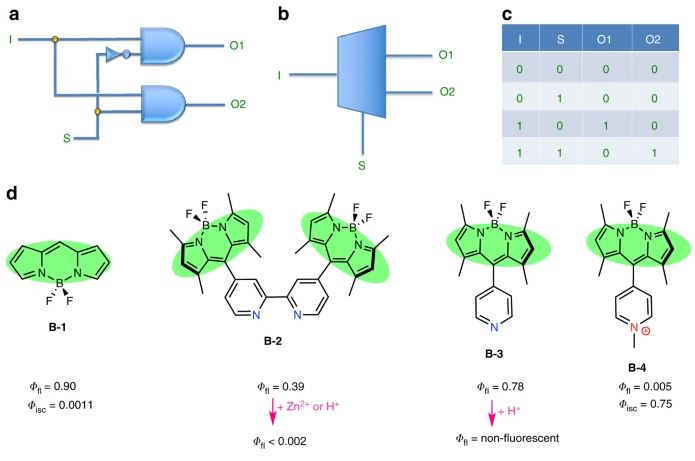
\includegraphics[width=7.5cm, height=5cm]{Ind. Natural/Imagen_02.jpg}
      \caption{Circuito Combinatorio DEMUX.}
      \label{Natural2} 
      \end{center}
\end{figure}
En la figura \ref{Natural2} se encuentra el circuito combinatorio DEMUX de \citeA{turan2018molecular} con símbolos de puerta lógica estándar. El trapezoide es un símbolo común para los circuitos MUX/DEMUX. Se tiene como entrada a S como la entrada de selección y dos salidas diferentes O1 y O2.

\vspace{1.5mm}
\subsubsection{\textbf{La reacción-difusión en un dominio 3D creciente de escamas de piel genera un autómata celular discreto: }}
En diferentes animales podemos ver diferentes patrones de colores en su piel debido a células pigmentarias que acumulan pigmentos negros, amarillos, rojos, etc. Las lagartijas, estos patrones en la piel de los animales son conocidos por generar varios patrones en escalas espaciales específicas. Se puede ver en la figura \ref{Natural3} el patrón juvenil de piel marrón con manchas blancas se transforma gradualmente, en el tronco dorsal del animal, en un patrón laberíntico adulto hecho de cadenas de escamas negras y verdes contrastantes. Debido a este cambio, \citeA{fofonjka2021reaction} pueden indicar que la red de escamas de piel en lagartos ocelados es un autómata celular probabilístico que calcula dinámicamente el patrón laberíntico adulto. Se concluye, que los autómatas celulares de Von Neumann, habiéndose sido considerados como sistemas computacionales abstractos, en realidad han sido generados por evolución biológica.
\begin{figure}[H]
 \begin{center}
       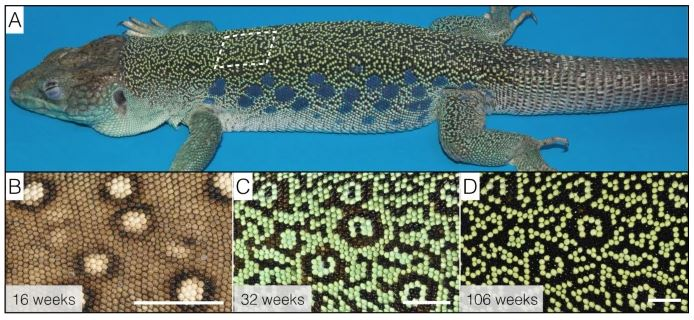
\includegraphics[width=7.5cm, height=5cm]{Ind. Natural/Imagen_03.jpg}
      \caption{Patrón de color de la ontogenia en lagartijas oceladas.}
      \label{Natural3} 
      \end{center}
\end{figure}
\subsection{\underline{\textbf{Industria Textil}}}

Con la evolución del hombre en paralelo ha ido evolucionando la tecnología satisfaciendo diferentes necesidades que requerimos y ayudándonos a que el trabajo arduo sea menor. Dicho esto, en la presente sección del artículo nos centraremos sobre el área de acuerdo a la industria textil donde gran parte del uso inicial que existe sobre la tecnología digital en la industria textil se ha enfocado en los métodos de fabricación e impresión de tejidos y fibras textiles donde se simplifica el trabajo además de exportar una mayor cantidad de diseños e imágenes en la impresión de telas mediante la producción automatizada en la industria y el uso de autómatas los cuales desde un determinado estado ejecutan una serie de pasos permitiendo así, llegar a un estado de meta deseado.

\vspace{2.5mm}
\subsubsection{\textbf{Autómatas textiles mediante autómatas celulares}}

Los autómatas celulares son modelos matemáticos y computacionales de manera discreta, sencilla y dinámica que están diseñados para un análisis de las propiedades mediante técnicas algebraicas y así modelar una máquina.
Los autómatas celulares pueden ser de las siguientes dimensiones: 
\begin{itemize}
\item Autómatas unidimensionales.
\item Autómatas bidimensionales.
\end{itemize}
Los autómatas unidimensionales permite que el número de regla puedan generarse aleatoriamente mientras que en los autómatas bidimensionales con 30 interacciones y valores aleatorios se podrían formar diferentes diseños textiles como observamos en la siguiente figura \ref{Textil1} la creación de diseños textil mediante autómatas celulares bidimensionales.
 \begin{figure}[H]
    \centering
    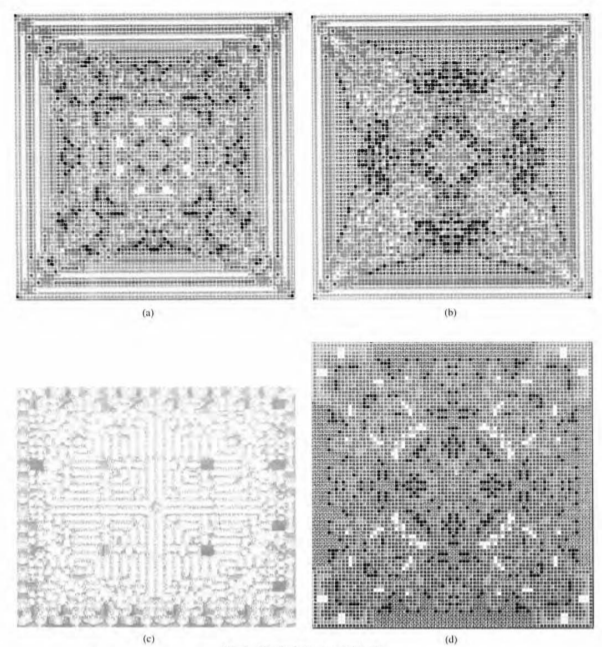
\includegraphics[width=7.5cm, height=5.5cm]{Ind. Tetxil/Aut. Textil Bidim..PNG}
    \caption{Diseño textil creado por autómatas celulares.}
    \label{Textil1} 
    \end{figure}
    \vspace{-2.6mm}
Tras el boceto del diseñador desarrollado en una computadora y este conectado a una máquina cortadora automatizada con celulares autómatas se generaría una gran variedad de diseños tras simples cálculos donde los patrones de los autómatas celulares bidimensionales y vecindad se generan interacciones irregulares lo cual se toman como diseños textiles.
\citeA{feijs2018cellular} nos permite ver a los autómatas celulares desde la perspectiva de la moda a lo cual lo llama un ``sistema complejo'' ya que es dinámico, recursivo y posee retroalimentación. La mayoría de modelos se basan en mecanismos de retroalimentación (Crane,1999) luego las empresas y grandes firmas de moda son las tendencias que compran su inteligencia para así, informen sus decisiones de diseño.
El diseño de autómatas celulares es que mediante determinadas reglas donde su comportamiento es difícil de predecir pero su salida debe ser un patrón tejido, es aquí donde sale Pied-de-paule donde en primera instancia era generar un autómata bidimensional pero se encontró patrones y reglas que sostenían a Pied-de-paule. 
En la figura \ref{Textil2} nos muestra como una regla de 9 maplets puede producir dos filas mas con una sola celda de color rojo oscuro. 
Formalmente los autómatas celulares,están definidos por:
\begin{itemize}
\item  La cuadrícula circular de células L.
\item  El conjunto de estados  Q = \{ - 2 , -1 , 0, 1, 2 \}.
\item  La estructura del entorno definida por r = 1.
\item  La regla de los 35 maplets
\end{itemize}

\begin{figure}[H]
    \centering
    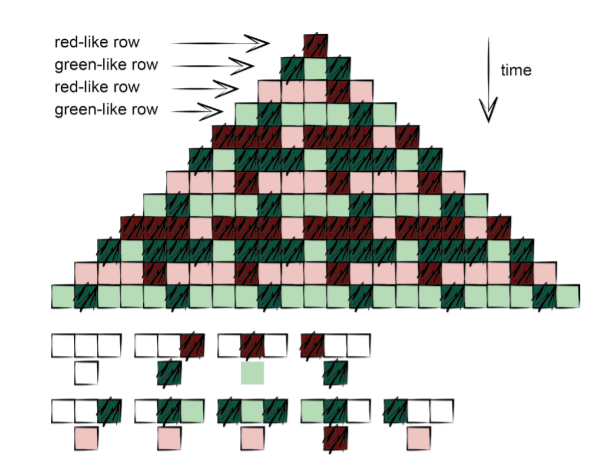
\includegraphics[width=7.5cm, height=5cm]{Ind. Tetxil/text2.PNG}
    \caption{Primeras 12 filas de un desarrollo Pied-de-poule (izquierda) y 9 maplets que son suficientes para el desarrollo de las dos primeras filas (t = 2 y t = 3) a partir de la fila inicial (t = 1).}
    \label{Textil2} 
    \end{figure}
\subsubsection{\textbf{Automatización en procesos textiles}}
En la industria textil se cuenta con diversos procesos industriales y servicios uno de los procesos de cuantificación de la estructura de compuestos textiles a partir de datos de tomografía es mediante los rayos X ya que nos brinda todo lo anterior mencionado mediante el modelamiento realista de los compuestos tras imágenes tridimensionales obtenidos con micro-CT para crear secciones transversales de un objeto físico que pueden usarse para recrear un modelo virtual sin destruir el objeto original, investigando su estructura tensorial y tras ello la determinación de orientaciones de fibras para obtener una mejor imagen de acuerdo a los componentes del material.
Según \citeA{STRAUMIT2015150} nos dice que los objetivos para un modelado eficiente nos implica el conocimiento de las orientaciones de las fibras que determinan las propiedades locales (anisotrópicas). Es por ello que la segmentación de imágenes se realiza mediante parámetros bidimensionales y umbrales de un determinado grado de anisotropía y valor permitiendo que los hilos se puedan distinguir , todo esto pasa automáticamente gracias a una estructura de vóxeles.

\subsubsection{\textbf{Sistemas para los procesos textiles}}
Uno de los softwares mas utilizados es el $"$Supervisory Control and data acquisiton$"$ donde se comunica a través de un campo de dispositivos para luego actuar de manera automática a continuación en la figura \ref{Textil3} se presenta el esquema básico SCADA donde hoy en día están evolucionando conteniendo sistemas integrados y pensados en resolver necesidades especificas cuantificando el tiempo y el consumo de la materia prima y almacenar la producción de cada telar teniendo en cuenta la velocidad y mas que todo controlar tanto la calidad como calidad de tela producida.
\begin{figure}[H]
\centering
    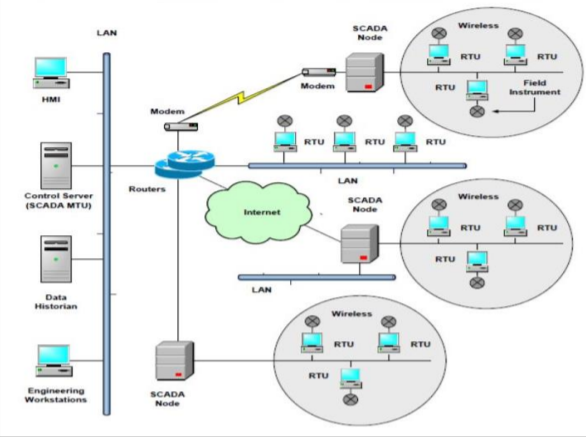
\includegraphics[width=7cm, height=4cm]{Ind. Tetxil/text3.PNG}
 \caption{Esquema básico de un SCADA}
 \label{Textil3}
\end{figure}


\vspace{2.5mm}
\subsection{\underline{\textbf{Industria Química}}}
\vspace{2.5mm}
 La tecnología ha evolucionado potencialmente en muchas ramas, así como en la química, se han desarrollado dispositivos electrónicos, que son un progreso para la industria química, aunque no puedan reemplazar los materiales básicos que un laboratorio posee, se ha implementado la tecnología en algunos procesos químicos, empleando los autómatas finitos.

\subsubsection{\textbf{Autómatas celulares en química e ingeniería química}}
Según \citeA{doi:10.1146/annurev-chembioeng-093019-075250}, los problemas de modelado de materiales y predicción de propiedades dependientes de la morfología, una aplicación de autómatas celulares en la resolución de problemas en química y tecnología química, implementados para modelar los procesos de difusión, disolución, erosión, corrosión, cristalización, adsorción e hidratación.Otra aplicación de CA en modelos híbridos, combinación de varios autómatas celulares, otros enfoques computacionales y método de modelado. Además la computación paralela de alto rendimiento aumenta le eficiencia de las autómatas celulares.

\vspace{2mm}
\subsubsection{\textbf{Cómo calcula la química: reconocimiento del lenguaje por autómatas químicos no bioquímicos. De los autómatas finitos a las máquinas de Turing}}

La computación esta presente en muchas áreas, tanto en dispositivos electrónicos como en sistemas vivos. Respecto a los sistemas vivos, según Conrad (1972) y Katz (2012), la bioquímica implementa la computación mediante las propiedades químicas de la materia orgánica, el proceso mecánico se da a través de reacciones químicas por lo que el resultado es químico. Según Rich(2008) y Katz(2012), el cálculo  es un proceso en el que la información pertenecientes a un lenguaje, conformado por símbolos de un alfabetos y con reglas que permiten a la máquina (autómata) procesar los símbolos y obtener una salida, una aceptación  o rechazo, en caso no pertenezca al lenguaje.
Este proceso se puede interpretar si consideramos las reacciones químicas como el resultado de eventos de reconocimiento molecular. Por lo que, se cuestiona si la complejidad de la bioquímica en el cálculo son necesarios, teniendo en cuenta la clasificación en jerarquía de Chomsky y que los idiomas son generado por gramáticas al imponerles restricciones gradualmente (Hopcroft et al., 2007), las gramáticas de Tipo-0 (no restringidas), Tipo-1 (lenguajes sensibles al contexto), Tipo-2 (lenguajes de libre contexto) y Tipo-3 (lenguaje regular). El Tipo-2 y 3, son un medio para leer secuencialmente la salida del programa y un indicador fisicoquímico autónomo que identifica patrones del lenguaje que reconoce la máquina. En este proceso, se introduce los símbolos al reactor, desde aquí todo el procesamiento y energía son químicas. Para \citeA{DUENASDIEZ2019514}, el objetivo del artículo es mostrar como las reacciones químicas pueden realizar la identificación de secuencias químicas, sin la bioquímica, mediante los autómatas en cálculos abstractos.

La figura \ref{Quimica1.1} muestra un autómata químico que está conformado de 3 sistemas: un reactor mezclado donde está presente la computación, un programador de entrada que alimenta la traducción en alícuotas químicas y un sistema de monitoreo que registre la respuesta de la máquina como una métrica química.

\begin{figure}[H]
 \begin{center}
       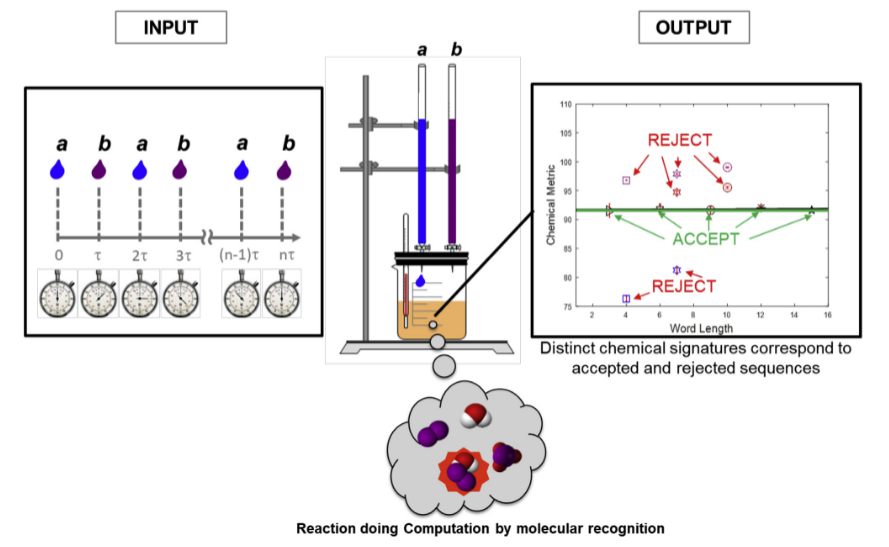
\includegraphics[width=8cm, height=5.5cm]{Ind. Química/A2.png}
      \caption{Máquina simple de dos estados descrita como (A)Representación gráfica dirigida de una máquina de estados finitos, (B) Red reguladora de genes de factores de transcripción e inductores reprimidos, y (C) Realización biomolecular del mismo GRN. Los círculos naranjas representan especies en transición, los círculos azules, especies estatales y los círculos verdes, especies censoras}
      \label{Quimica1.1} 
      \end{center}
\end{figure}

\subsubsection{\textbf{Marco para la ingeniería de máquinas de estados finitos en redes reguladoras de genes}}
Las máquinas de estados finitos son fundamentales para los núcleos de algunos modelos de computación, son comúnmente usados en modelos de desarrollo en organismo multicelulares, aún así no se sabe como las células pasan de un estado a otro y si las partes existentes son suficientes para emplear máquinas de estados finitos en células vivas, incluso aún no se comprende cómo se puede realizar comportamientos multicelulares complejos empleando la coordinación de los estados de las células con la señalización, crecimiento y división. Por lo que, según \citeA{doi:10.1021/sb4001799}, el artículo describe un método  en el cual una máquina de estados finitos puede ser construida empleando una red diseñada de factores de transcripción, mostrando la equivalencia matemática de máquinas de estados finitos como modelo booleano de redes reguladora de genes.
Adicionalmente, presenta un diseño para la detección de borde de microcolonia bacteriana sintética, la cual mediante las máquinas puede ser usadas junto a la señalización celular con el fin de construir comportamientos multicelulares innovadores.

La figura ~\ref{Quimica2} muestra el proceso en la máquinas de estados finitos para redes reguladoras de genes.
\begin{figure}[H]
 \begin{center}
       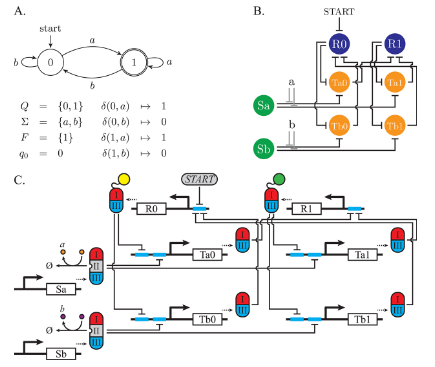
\includegraphics[width=8cm, height=7cm]{Ind. Química/A3.png}
      \caption{Máquina simple de dos estados descrita como (A)Representación gráfica dirigida de una máquina de estados finitos, (B) Red reguladora de genes de factores de transcripción e inductores reprimidos, y (C) Realización biomolecular del mismo GRN. Los círculos naranjas representan especies en transición, los círculos azules, especies estatales y los círculos verdes, especies censoras}
      \label{Quimica2} 
      \end{center}
\end{figure}

El modelado de redes reguladoras de genes se especifican mediante una lista ordenada finita de elementos,
\begin{equation}G=(G_{V},G_{U})\end{equation}
\begin{equation}G_{V}=(V,E_{r},E_{a})\end{equation}
\begin{equation}G_{U}=(U,I_{r},I_{a})\end{equation}
 \begin{itemize}
     \item \begin{math}G_{V}\end{math}: gráfico de red de genes internos
     \item \begin{math}V\end{math}: conjunto finito de productos génicos.
     \item \begin{math}G_{U}\end{math}: gráfico de señales.
 \end{itemize}
 La red reguladora de genes es comúnmente representada como un grafo dirigido, donde V y U son los vértices, \begin{math}E_{r}\end{math} y \begin{math}E_{a}\end{math} son borde de represión y activación que conectan nodos en V y \begin{math}I_{r}\end{math} y \begin{math}I_{a}\end{math} son la represión 
 de señales dirigidas que conectan nodos en U.
 
 
 %\subsubsection{\textbf{Una simulación de autómatas celulares estocásticos de oscilaciones químicas en sistemas pequeños}}
%Según \citeA{doi:10.1063/1.5051550}, proponen simular una reacción química mediante el método de autómata celular estocástico en sistemas pequeños, los cuales están divididos en células independientes de pocas moléculas. Durante la investigación, descubrieron que la distribución de partículas, aparte de las de Poisson, son capaces de sur
%--------------------------------------------------------------------
\vspace{2mm}
\subsection{\underline{\textbf{Industria Ambiental}}}
\vspace{2mm}
\subsubsection{\textbf{Un marco integrado para el dimensionamiento y la gestión energética de híbridos}}
La energía híbrida es la que utiliza más de una fuente renovable para lograr producir energía. Gracias a muchos de los beneficios que esta ofrece es necesario que se aproveche al máximo. De ahí la importancia del ahorro de costes y su uso eficiente. Ante ello, \citeA{energiahibrida} presentó un marco integrado para hallar una gran combinación entre la estrategia de gestión de tamaño y energía para este tipo de sistema. Lo más resaltante de este informe es que, usa los autómatas finitos para el desarrollo de múltiples estrategias de gestión de la energía.\par 
Para ilustrar cómo es un subsistema en HES; \citeA{energiahibrida} menciona que el HES incluye PV, sistema de energía de batería (BES), electrolizador (EL), celda de combustible (FC), tanque de hidrógeno (HT) y generador diesel (DSL); puede tratarse como DES(Sistemas de eventos discretos) y modelarse en FA (Autómatas finitos), se presenta un ejemplo de BES(Sistema de energía de batería) en la figura ~\ref{Amb-1}. El BES en HES tiene cuatro estados: carga, descarga, inactivo y APAGADO. Los círculos en la figura representan los estados, mientras que las transiciones son los eventos o las condiciones de operación. El estado con círculos dobles simboliza el estado marcado, que también es el estado final, que indica la finalización de la operación BES.
\begin{figure}[H]
 \begin{center}
       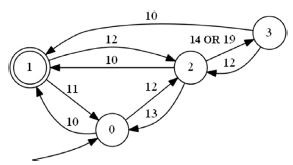
\includegraphics[width=7cm, height=3cm]{Ind. Ambiental/1.JPG}
      \caption{Un ejemplo ilustrado sobre la implementación de BES usando FA.}
      \label{Amb-1} 
      \end{center}
\end{figure}
Luego de haber realizado la comparación entre los resultados del marco propuesto y los resultados del enfoque de dimensionamiento analítico y económico. \citeA{energiahibrida}, demostró que el tamaño de la fotovoltaica se reduce de $140 kW$ a $60 kW$ cuando se usa el marco integrado y por lo tanto el tamaño del electrolizador y el tanque de hidrógeno se reduce a la mitad. Además, se logró una reducción en las horas de trabajo del generador diesel en un 35\% y en el costo nivelado de la energía en un 40\%.
\vspace{2.5mm}
\subsubsection{\textbf{Simulando la propagación de incendios forestales y la extinción de incendios utilizando autómatas celulares}}
Frente al problema de la neblina transfronteriza que presenta el sudeste asiático, se simula un modelo físico de la propagación y extinción del fuego, en el contexto de Dumai, Indonesia puesto que, esta ciudad es uno de los que más contribuye significativamente a este problema.\par
\citeA{neblinasimular} presentan un modelo que tiene como objetivo proporcionar perspectivas sobre la persistencia de los incendios forestales a pesar de los esfuerzos de extinción. Este modelo aplica autómatas celulares para predecir y analizar los efectos de las estrategias de intervención contra incendios, teniendo en cuenta la dinámica espacial y la propagación del fuego.
%-----------------------------
\begin{figure}[H]
\centering
  \subfigure[Superficie quemada real de Dumai del 2014]
   {
    \label{Amb-2}
    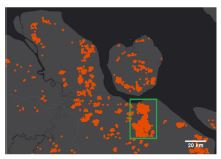
\includegraphics[width=4cm, height=3cm]{Ind. Ambiental/2.JPG}
    }
  \subfigure[Simulación de Montecarlo en Dumai]{
   \label{Amb-3}
    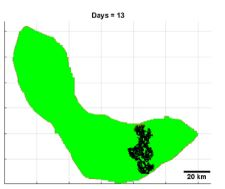
\includegraphics[width=4cm, height=3cm]{Ind. Ambiental/3.JPG}}
 \caption{Resultados}
 \label{figuras1-2}
\end{figure}
%-----------------------------
De la Figura ~\ref{Amb-2}, las regiones rojas denotan un área quemada mientras que las regiones grises denotan la vegetación restante. La región de interés está resaltada en un recuadro verde, y de la Figura ~\ref{Amb-3} las regiones negras denotan el área quemada; las regiones rojas denotan áreas que aún están ardiendo; las regiones verdes denotan la vegetación restante.

El área del bosque se discretiza en una gran cuadrícula, sobre la que se apoya un autómata celular bidimensional (CA). Las celdas del bosque pueden estar en uno de cuatro estados en cualquier momento: El estado ``combustible'', la vegetación que puede incendiarse; el estado ``ardiendo'', el combustible que se está quemando actualmente; el estado ``vacío'', un área de tierra sin combustible o fuego y el estado ``quemado'', al combustible que ha dejado de arder. Las áreas sin vegetación están marcadas como ``vacías''.\par La evolución de los estados de las células a lo largo de los intervalos de tiempo se rige por un conjunto de reglas que modelan el comportamiento de la propagación del fuego. Se puede razonar que, en primer lugar, una celda quemada permanecerá encendida, ya que la escala de tiempo de los incendios forestales suele ser demasiado corta para que se produzca la regeneración de la vegetación; en segundo lugar, las células en llamas se quemarán después de un paso de tiempo, con la duración física de un paso de tiempo elegido apropiadamente; y en tercer lugar, una celda de combustible junto a una celda en llamas puede incendiarse con cierta probabilidad.

Por lo que, \citeA{neblinasimular} logró
predecir computacionalmente la propagación del fuego a partir de los datos iniciales de las observaciones lo que permitirá la optimización anticipada de los esfuerzos de extinción de incendios y puede permitir una supresión más eficaz de la actividad del fuego con los recursos disponibles, como el bombardeo de agua.

\vspace{2.5mm}
\subsubsection{\textbf{Construcción de un modelo para el reconocimiento de patologías morfoestructurales en tejidos animales}}
Debido a la gran demanda de métodos y modelos para el diagnóstico histológico automatizado de enfermedades en animales, \citeA{animales} proponen la creación de sistemas expertos de análisis histológico que puedan ser utilizados en medicina veterinaria clínica y de esta forma poder contribuir en la formación avanzada de patólogos veterinarios.\par
Así, muestran la posibilidad de utilizar la teoría de autómatas finitos para la construcción del dispositivo - analizador histológico, para realizar el análisis histológico. Paraeste análisis utilizaron el reconocimiento de imágenes de cambios morfofuncionales en tejidos de roedores en el ejemplo especifico del cerebro blando de una rata dañada por infección por clamidia. 
\begin{figure}[H]
 \begin{center}
       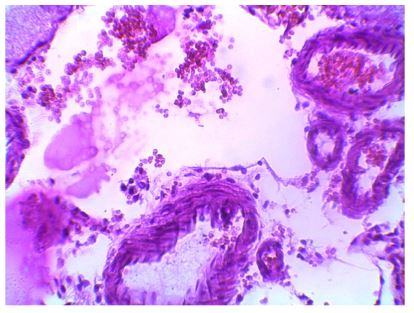
\includegraphics[width=
       3cm, height=2cm]{Ind. Ambiental/4.JPG}
      \caption{Patología de la piamadre de una rata dañada por clamidia. x 400.}
      \label{Amb-4} 
      \end{center}
\end{figure}
Para este reconocimiento de imágenes, \citeA{animales} sugieren la utilización de tecnologías de redes neuronales informáticas basadas en perceptores multicapa. De esta manera, demostraron que, se puede hacer uso de tecnologías de redes neuronales para el reconocimiento de indicadores de patología durante el análisis histológico de cambios morfoestructurales en tejidos animales.

\vspace{2.5mm}
\subsubsection{\textbf{Difusión de información de riesgo de neblina basada en autómatas celulares}}
Por los diversos efectos negativos que presenta el riesgo de neblina, estas pueden llegar a propagarse más rápido, sin embargo, no existen estudios donde se investigue el periodo completo o ciclo de eventos de difusión, lo que genera que muchas personas no se enteren y provoca efectos negativos enormes. 
Por ello, \citeA{neblina} utilizan el modelo de simulación de difusión que se muestra en la figura \ref{Amb-5} basado en autómatas celulares para evaluar la difusión de información sobre el riesgo de neblina.
\begin{figure}[H]
 \begin{center}
       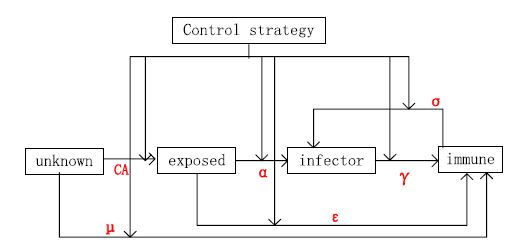
\includegraphics[width=
       8cm, height=3cm]{Ind. Ambiental/5.JPG}
      \caption{Estrategia de control de difusión de información sobre riesgos de neblina}
      \label{Amb-5} 
      \end{center}
\end{figure}
\citeA{neblina} concluye que, todavía hay muchas deficiencias en la simulación de todo el ciclo de vida de la difusión de información sobre riesgos de neblina. Para los vecinos del autómata celular, solo se seleccionó el tipo Von Neuman pero no el tipo Moore. La consideración de la influencia de los vecinos circundantes puede no ser exhaustiva. En las reglas de evolución, se consideraron las condiciones de contorno, pero se ignoraron las posiciones de los vértices.\par
Para lograr un control efectivo de la propagación de la información sobre el riesgo de neblina, se tomaron medidas de control fuertes y débiles para cada tipo de individuos, y se aumentó la inmunidad de los desconocidos y los acechadores para el control del tipo individual.
%--------------------------------------------------------------------
\vspace{2.5mm}
\subsection{\underline{\textbf{Industria Tecnológica}}}
\vspace{2.5mm}
\subsubsection{\textbf{Autómata finito que utiliza la optimización de colonias de hormigas con árbol de expansión}}

    Según \citeA{aliyu2021management}, propone en su investigación de autómatas finitos utilizando Ant Colony Optimization con Spanning Tree (FAACOST), un concepto de aprendizaje automático para administrar los recursos de la nube en un entorno de varios niveles. Teniendo como objetivo general el minimizar el consumo de energía, a través de datos, apalancamiento de ubicación y consolidación de máquinas virtuales (VM).
    
    Comparándose así, la eficiencia de la técnica propuesta en cuatro métricas de rendimiento: \textit{aprendizaje automático, naturaleza dinámica, escalabilidad y QoS}. Basado en
    extensos experimentos realizados, FAACOST registró un consumo de energía de $132 w$ con 20 tareas en comparación a las técnicas de referencia que consumieron $363 w$.

    \begin{figure}[H]
    \begin{center}
    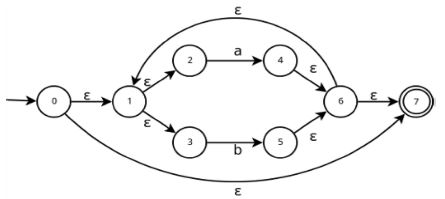
\includegraphics[width=6cm, height=2.4cm]{Ind.Tecnolo/Ant.JPG}
    \caption{TSG de (a/b)*.}
    \label{Tec.1} 
    \end{center}
    \end{figure}
    
    Las hormigas artificiales en el TSG (Transition state graph) (Figura ~\ref{Tec.1}) pueden tener cualquier estado inicial y realizar transiciones para el procesamiento de tareas en un data centers, DC o centro de datos. 
    Los resultados experimentales muestran que ``FAACOST logra el número óptimo de máquinas físicas(PM) y es más eficiente desde el punto de vista energético''  \cite[p.~11]{aliyu2021management}.
    
\vspace{2.5mm}    
\subsubsection{\textbf{Revisión sistemática de arquitecturas de hardware escalables para la coincidencia de patrones en la seguridad de la red}}    
    Los algoritmos y técnicas de coincidencia de patrones se implementan ampliamente en un sistema de detección de intrusiones en la red. Existe una gran cantidad de arquitecturas de hardware de coincidencia de patrones escalables con varios parámetros de diseño.

    Por lo que, \citeA{imran2021systematic} en su estudio de investigación más reciente, relacionado con la implementación de hardware escalables de algoritmo técnicas de coincidencia de patrones, a través de una revisión sistemática de la información, seleccionó 49 estudios de investigación; los cuales se clasificaron, Figura ~\ref{Tec.2}, en cadenas, algoritmos y expresiones regulares de coincidencia y también fueron analizados.

    \begin{figure}[H]
    \begin{center}
    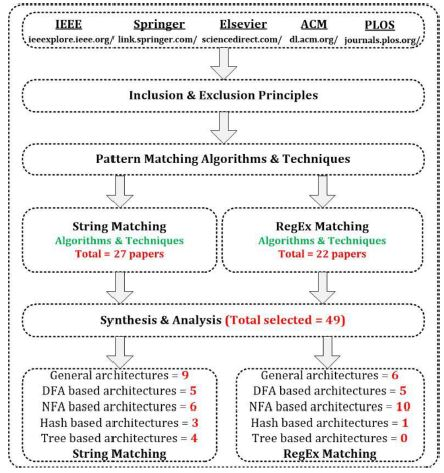
\includegraphics[width=7cm, height=5.5cm]{Ind.Tecnolo/Patron.JPG}
    \caption{Descripción general del enfoque del patrón de coincidencias.}
    \label{Tec.2} 
    \end{center}
    \end{figure}
    
    Siendo el autómata finito (FA), una de las técnicas destacadas en el módulo de detección de eventos de coincidencia de patrones. Debido a que, funciona como una máquina de estados finitos (FSM) para reconocer los patrones almacenados dentro de los flujos de caracteres de entrada, dependiendo su cálculo de sus cinco tuplas.
    
    Obteniéndose que los enfoques DFA, Autómata finito Determinista, y NFA, Autómata finito No Determinista, son utilizados con frecuencia por investigadores/diseñadores, ya que requieren una \textbf{menor utilización de la memoria} y dan como resultado una \textbf{mayor velocidad de procesamiento}. Además, se identificaron algunas soluciones completas de hardware, donde la captura, decodificación y las unidades de preprocesamiento 
    se implementan al mismo tiempo. De esa manera, para \cite[p.~16]{aliyu2021management}, esto guiará a los investigadores en: 
    \begin{enumerate}
        \item Una arquitectura de hardware, de acuerdo con diferentes enfoques de implementación. 
        \item Arquitecturas de coincidencia de patrones de uno varios caracteres con diferentes configuraciones.
        \item Una arquitectura de hardware para la implementación de IDS (Intrusion Detection System) o sistema de detección de intrusiones completos.
    \end{enumerate}

\vspace{2.5mm}    
\subsubsection{\textbf{Mecanismo de control distribuido y paralelo para la autoconfiguración de robots modulares utilizando sistemas L y autómatas celulares}}

    Para la autoconfiguración distribuida de robots Modular Self-Reconfigurable (MSR), uno de los inconvenientes es la contradicción entre la información limitada de los módulos descentralizados y la estructura global bien organizada.
    
    Por lo que \citeA{zhu2017distributed} precisa un mecanismo híbrido al combinar sistemas Lindenmayer (sistemas L) que describen la estructura topológica como objetivo de configuración y Autómatas celulares (CA) para la planificación del movimiento local de módulos individuales.
    
    Según su investigación, los módulos independientes realizan la planificación del movimiento por Cellular Automata en paralelo. Este mecanismo distribuido es resistente a fallas de módulos, escalable a diferentes números de módulo y convergente a objetivos de reconfiguración predefinidos.
    
    Los resultados estadísticos que se observa en la Figura  ~\ref{Tec.3}, muestra cómo los pasos de tiempo para la convergencia aumenta a medida que aumenta el número de módulos y 
    el número de pasos de tiempo para la autoconfiguración crece linealmente con la
    número de módulos. Este aumento lineal significa un gran avance en relación con el
    crecimiento exponencial en la planificación óptima de la reconfiguración.
    
    \begin{figure}[H]
    \begin{center}
    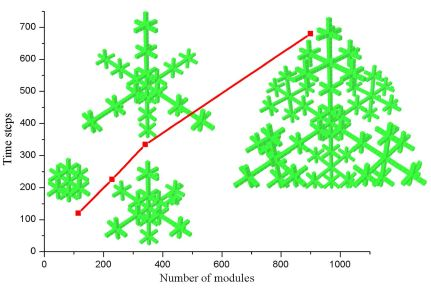
\includegraphics[width=6cm, height=4cm]{Ind.Tecnolo/Rob.JPG}
    \caption{La escalabilidad a los números de módulo de la autoconfiguración.}
    \label{Tec.3} 
    \end{center}
    \end{figure}

   “El mecanismo propuesto es eficiente, robusto, escalable y convergente, que se verifica mediante diversas simulaciones, estadísticas y resultados" \cite[p.~29]{zhu2017distributed}.

\vspace{2.5mm}  
\subsubsection{\textbf{CADbots: aspectos algorítmicos de la manipulación de materia programable con autómatas finitos}}
    \citeA{fekete2021cadbots}, presenta métodos algorítmicos para evaluar y manipular un colectivo de partículas por un autómata finito que no puede almacenar significantes cantidades de datos, ni realizar cálculos complejos, y se limita a posibles operaciones físicas.
    
    Por lo que, proporciona una caja de herramientas para que se lleve a cabo tareas fundamentales 
    en una determinada disposición de partículas, utilizando la propia disposición como dispositivo de almacenamiento, similar a una máquina de Turing de dimensiones superiores con propiedades geométricas.
    
    \begin{figure}[H]
    \begin{center}
    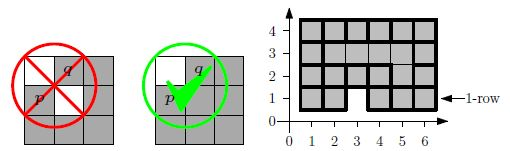
\includegraphics[width=7.8cm, height=2.5cm]{Ind.Tecnolo/cad.JPG}
    \caption{Configuración del robot para la cuadrícula.}
    \label{Tec.4} 
    \end{center}
    \end{figure}
    
    Considerándose un solo robot que actúa como un autómata finito determinista. El robot se mueve en la cuadrícula $(infinita) G = ({Z}^2 , E)$ con bordes entre todos los pares de nodos que están dentro de la distancia unitaria usando la métrica de Manhattan. Los nodos de $G$ se llaman píxeles. Cada píxel se encuentra en uno de dos estados: está vacío u ocupado, Figura ~\ref{Tec.4}.
    
    Además, $P$ de $N$ partículas de forma cuadrada, en la que un solo robot de estado finito puede realizar un conjunto limitado de operaciones; donde se tuvo por objetivo desarrollar los primeros enfoques para evaluar y modificar el arreglo definiendo secuencias de transformaciones y proporcionando métricas para tales secuencias. 
%--------------------------------------------------------------------
\vspace{2.5mm}
\section{\textbf{Conclusiones}}
    Respecto a los autómatas finitos, celulares y moleculares en la industria natural, se puede ver su importancia y que estos autómatas están vinculados con incluso la evolución de seres vivos. Los autómatas sirven para un mayor entendimiento de los patrones y sistemas biológicos dentro de la naturaleza, además también de su uso para innovar como es el caso del circuito combinatorio DEMUX, también podemos ver la presencia de estos autómatas celulares dentro de la biología de diferentes animales. Esto deja como conclusión la importancia de estos autómatas dentro de la naturaleza, donde cada sistema creado por la misma naturaleza y vida está perfectamente estructurado para tener una función en específico, además también de su uso en la innovación de circuitos combinatorios en contra de enfermedades como el cáncer.
    
    Del mismo modo, en la industria textil para un mejor progreso de este sector se hace el uso de diferentes herramientas, donde se ha podido evidenciar en el presente artículo la utilización de autómatas con sus expresiones regulares , así mismo se ha podido evidenciar el uso de los autómatas celulares  lo cual permite el diseño de los tejidos elevando así los modelos de una pieza textil, además de contar con diversos softwares el cual hoy en día van evolucionando y que también se obtiene resultados prometedores tanto como diseño, procesamiento y automatización en la industria textil.

    Respecto al uso de autómatas finitos en la industria química, se ha evidenciado su aporte a esta ciencia en la resolución y simulación de ciertos procesos como se menciona en los  artículos citados, por lo que, es un avance importante aunque no pueda reemplazar los experimentos del laboratorio o sus materiales, es de gran ayuda para simular procesos y obtener resultados similares.

    En la industria ambiental es fundamental la utilización de la teoría de lenguajes formales y autómatas ya que se demostró que gracias a ella,  el tamaño de la fotovoltaica se redujo de $140 kW$ a $60 kW$ cuando se usa el marco integrado, así también se logró predecir computacionalmente la propagación del fuego a partir de los datos iniciales de las observaciones lo que permitirá la optimización anticipada de los esfuerzos de extinción de incendios, como también se demostró que se puede hacer uso de tecnologías de redes neuronales para el reconocimiento de indicadores de patología durante el análisis histológico de cambios morfoestructurales en tejidos animales.
    
    Por otro lado dentro de la industria tecnológica y tomando en cuenta a los autómatas finitos, se expuso que son empleados para evaluar el procesamiento del texto a través de un DFA, situaciones del comportamieno de los robots, la inteligencia artificial y el aprendizaje automático, empleando algoritmos eficientes de gran trascendencia en los que se tiene como objetivo usar menos recursos computacionales.

%--------------------------------------------------------------------
\bibliographystyle{apacite}
\bibliography{Referencias}

\end{document}
